\documentclass[a4paper,12pt]{article}
\usepackage{graphicx}
\usepackage{amsmath}
\usepackage{amsfonts}
\usepackage{amssymb}
\usepackage{geometry}
\usepackage{booktabs}
\usepackage{float}
\usepackage{hyperref}
\usepackage{caption}
\usepackage{fancyhdr}
\usepackage{listings}
\usepackage{subcaption}
\usepackage{xcolor}
\usepackage{pgfplots}
\usepackage{longtable}

\definecolor{codegray}{rgb}{0.95,0.95,0.95}
\definecolor{codegreen}{rgb}{0,0.6,0}
\definecolor{codeblue}{rgb}{0,0,0.6}
\definecolor{codepurple}{rgb}{0.58,0,0.82}

% Code block styling to look professional
\lstdefinelanguage{json}{
    basicstyle=\ttfamily\footnotesize,
    commentstyle=\color{codegreen},
    stringstyle=\color{codepurple},
    keywordstyle=\color{codeblue},
    showstringspaces=false,
    breaklines=true,
    backgroundcolor=\color{codegray},
    frame=single,
    rulecolor=\color{lightgray}
}

\lstdefinestyle{pythonstyle}{
    language=Python,
    backgroundcolor=\color{codegray},   
    commentstyle=\color{codegreen},
    keywordstyle=\color{codeblue},
    numberstyle=\tiny\color{gray},
    stringstyle=\color{codepurple},
    basicstyle=\ttfamily\footnotesize,
    breakatwhitespace=false,         
    breaklines=true,                 
    captionpos=b,                    
    keepspaces=true,                 
    numbers=left,                    
    numbersep=5pt,                  
    showspaces=false,                
    showstringspaces=false,
    showtabs=false,                  
    tabsize=4,
    frame=single,
    rulecolor=\color{lightgray}
}

\geometry{margin=1in}
\hypersetup{
    colorlinks=true,
    linkcolor=blue,
    filecolor=magenta,      
    urlcolor=cyan,
}
\pagestyle{fancy}
\fancyhf{}
\fancyhead[L]{Final Project}
\fancyhead[R]{\thepage}

\begin{document}

\begin{titlepage}
    \centering
    \vspace*{1cm}
    
    {\Huge \textbf{Data Networks}}\\[1.5cm]

    \begin{figure}[ht]
        \centering
        % Replace with actual university logo
        
\includegraphics[width=0.4\textwidth]{Images/logo.jpg}
    \end{figure}

    \vspace{1cm}
    {\Large \textbf{BitTorent, A peer to peer file sharing system}}\\[0.5cm]

    \textbf{Department of Electrical Engineering} \\ 
    Sharif University of Technology \\[0.5cm]
    \textbf{Instructor: Dr. Mohammad Reza Pakravan} \\[2.0cm]
    
    \textbf{Submitted by:} \\[0.5cm]
    {\Large Amirali Yazdiani - 402102765} \\[1.5cm]

    \vfill
    \textbf{Date:} \\
    Aug 2026
\end{titlepage}

\newpage
\tableofcontents
\newpage

\section{Torrent File Generation}
To make the configuration process user friendly and human readable, the initial configurations for the torrents were written in JSON format. 
This allows for easy modification of the target files and piece lengths without dealing with raw binary data.

\begin{lstlisting}[language=json, numbers=none, caption={Single File Torrent Example}] 
{
  "announce": "http://127.0.0.1:8000/announce",
  "info": {
    "name": "Transferring_These_Files/sample3.png",
    "length": 1455741,
    "piece length": 262144,
    "pieces": ""
  }
}
\end{lstlisting}

\begin{lstlisting}[language=json, numbers=none, caption={Multi File Torrent}] 
{
  "announce": "http://127.0.0.1:8000/announce",
  "info": {
    "name": "Transferring_These_Files",
    "piece length": 262144,
    "pieces": "",
    "files": [
      {
        "length": 1116449,
        "path": ["sample1.png"]
      },
      {
        "length": 1455741,
        "path": ["sample2.png"]
      }
    ]
  }
}
\end{lstlisting}

Using the \texttt{torrent\_generator.py} script, these JSON files are parsed, the actual physical files are read, and their SHA-1 hashes are computed for each piece. 
The script then generates the final \texttt{.txt} file encoded in the Bencode format.

\textbf{Why Bencode?} While JSON is easy to read, the BitTorrent protocol mandates Bencoding. This is because Bencoding explicitly supports arbitrary binary data (like the concatenated SHA-1 hashes in the \texttt{pieces} field) 
and ensures a deterministic serialization order. This determinism is critical because any slight change in formatting would alter the \texttt{info\_hash}, completely breaking peer discovery in the network.

\section{Tracker Web Service}
The Tracker acts as the central directory of the BitTorrent ecosystem. 
It does not store or transfer any of the actual files. Its sole responsibility is to track which peers are currently in the swarm and facilitate their discovery.

In this implementation, the tracker operates as a multithreaded HTTP server. 
It maintains a dictionary (\texttt{swarm\_db}) where the keys are the torrent \texttt{info\_hash}es and the values are lists of active peers (IP and Port). When a peer connects to the \texttt{/announce} endpoint, 
the tracker handles three specific events:
\begin{itemize}
    \item \textbf{Started:} Adds the peer to the swarm database or updates its port if it already exists.
    \item \textbf{Completed:} Marks the peer as a "seeder".
    \item \textbf{Stopped:} Gracefully removes the peer from the database so other peers do not attempt to connect to a dead node.
\end{itemize}
The tracker then responds with a bencoded dictionary containing the swarm statistics and the list of available peers.

\section{Peer Client Operation}
The peer client is the core component responsible for downloading and seeding files. 
The execution flow follows a strict, step by step procedure:
\begin{enumerate}
    \item \textbf{Initialization:} The peer generates a unique 20 byte identifier (starting with \texttt{-AA0001-}) 
    to represent itself in the swarm.
    \item \textbf{Port Binding:} It attempts to open a TCP listening socket starting at port 6881. If the port is in use, it sequentially tries the next ports up to 6889.
    \item \textbf{Tracker Communication:} The peer sends an HTTP GET request to the tracker's announce URL to register itself and retrieve a list of other active peers.
    \item \textbf{Handshake:} Upon receiving peer addresses, it initiates direct TCP connections and performs the 68 byte BitTorrent handshake to verify protocol compatibility and the \texttt{info\_hash}.
    \item \textbf{Data Exchange:} Peers exchange bitfield messages to declare which pieces they have. The client then sends \texttt{INTERESTED} messages and requests file pieces sequentially using \texttt{REQUEST} messages, 
    saving them directly to a local buffer and verifying their SHA-1 hashes upon receipt.
\end{enumerate}

\section*{The BitTorrent Handshake Protocol}

The BitTorrent protocol mandates a strict 68 byte handshake as the first message transmitted when two peers establish a connection. This message is critical for verifying protocol compatibility and ensuring both peers are interested 
in the same torrent file.

\begin{figure}[H]
    \centering
    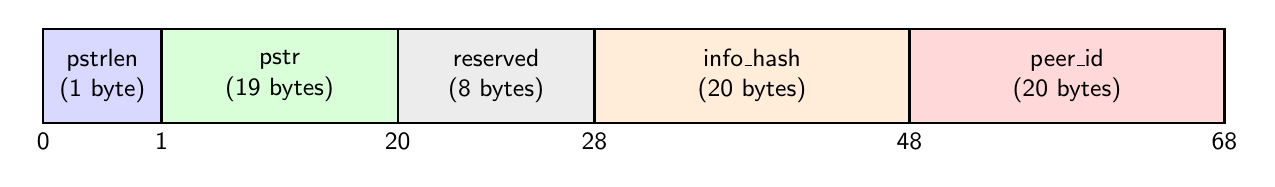
\begin{tikzpicture}[every node/.style={font=\sffamily\small}]
        % Blocks
        \draw[fill=blue!15, thick] (0,0) rectangle (1.5,1.2) node[midway, align=center] {pstrlen\\(1 byte)};
        \draw[fill=green!15, thick] (1.5,0) rectangle (4.5,1.2) node[midway, align=center] {pstr\\(19 bytes)};
        \draw[fill=gray!15, thick] (4.5,0) rectangle (7,1.2) node[midway, align=center] {reserved\\(8 bytes)};
        \draw[fill=orange!15, thick] (7,0) rectangle (11,1.2) node[midway, align=center] {info\_hash\\(20 bytes)};
        \draw[fill=red!15, thick] (11,0) rectangle (15,1.2) node[midway, align=center] {peer\_id\\(20 bytes)};
        
        % Byte offsets
        \node[below] at (0,0) {0};
        \node[below] at (1.5,0) {1};
        \node[below] at (4.5,0) {20};
        \node[below] at (7,0) {28};
        \node[below] at (11,0) {48};
        \node[below] at (15,0) {68};
    \end{tikzpicture}
    \caption{Structure of the 68-byte BitTorrent Handshake Message}
    \label{fig:handshake}
\end{figure}

As illustrated in Figure \ref{fig:handshake}, the 68 bytes are structured into five distinct sections:

\begin{enumerate}
    \item \textbf{pstrlen (1 Byte):} The string length of the protocol identifier. For the standard BitTorrent protocol, this value is always \texttt{19} (0x13 in hexadecimal).
    
    \item \textbf{pstr (19 Bytes):} The string identifier of the protocol. It is strictly encoded as the string \texttt{"BitTorrent protocol"}.
    
    \item \textbf{reserved (8 Bytes):} Eight reserved bytes set to zero (\texttt{0x00}). These bytes are reserved for future extensions.
    
    \item \textbf{info\_hash (20 Bytes):} The 20 byte SHA-1 hash of the \texttt{info} key from the bencoded metainfo (\texttt{.torrent}) file. This verifies that both peers are attempting to transfer the exact same swarm data.
    
    \item \textbf{peer\_id (20 Bytes):} A unique 20 byte string randomly generated by the client upon startup to identify itself within the swarm.
\end{enumerate}

\section{Centralized Logger}
To properly monitor the asynchronous nature of peer to peer networks, a custom \texttt{logger.py} was implemented. 
Standard console outputs are insufficient when multiple threads and clients are running concurrently. 

The logger dynamically creates isolated log files for both the Tracker and each individual Peer. 
It categorizes every event (handshakes, ping successes, errors) and records them with precise timestamps in a structured format containing a header (metadata) and a body (tabulated event history).

\section{Web Based Dashboard (AI Assisted)}
To better comprehend the real time topological changes and traffic within the network, a graphical dashboard was developed using HTML, JavaScript, and the Vis.js library. 

The dashboard connects to the tracker's API to visually map the swarm and animate network events such as \texttt{PING}, \texttt{PONG}, \texttt{PIECE}, and \texttt{REQ} messages, providing a highly intuitive understanding of the underlying protocol mechanics.

\textit{It should be noted that this graphical interface was developed with the assistance of Artificial Intelligence.} 

\section{Unimplemented Features \& Future Work}
While the core file sharing mechanics are fully functional, some advanced BitTorrent specifications were omitted in this implementation:
\begin{itemize}
    \item \textbf{Rarest First Algorithm:} The current system fetches pieces sequentially rather than prioritizing the rarest pieces available in the swarm.
    \item \textbf{Choking/Unchoking Logic:} Advanced bandwidth optimization algorithms are not fully enforced.
\end{itemize}

\textbf{GitHub Repository \& Parallel Download Branch:}\\
The entire source code is available in the following GitHub repository:\\
\url{https://github.com/amirali83/Project} 

An attempt was made to implement simultaneous multi peer downloading (Swarm downloading). This work is located in a separate branch named \texttt{parallel\_download}. 
However, this branch is currently unstable and suffers from synchronization and state management bugs, thus it is not included in the main implementation.

\section{Step by Step Execution Guide}
To execute the project and observe the file sharing process locally, follow these exact steps:

\begin{enumerate}
    \item \textbf{JSON Configuration:} It is highly recommended \textbf{not} to modify the \texttt{torrent1.json} and \texttt{torrent2.json} files. 
    They are already strictly linked to the existing local files and correctly demonstrate both single file and multi file architectures. Adding a third 
    torrent would require hardcoding logic changes within the peer script.
    \item \textbf{Generate Bencoded Torrents:} Open a terminal and run the generator script to convert the JSON configurations into the final bencoded \texttt{.txt} files required by the system:
    \begin{lstlisting}[language=bash, numbers=none]
    python torrent_generator.py
    \end{lstlisting}
    \item \textbf{Start the Tracker:} In a new terminal, execute the tracker server. Once running, you can open a web browser and navigate to \texttt{http://127.0.0.1:8000/dashboard} to access the graphical visualization.
    \begin{lstlisting}[language=bash, numbers=none]
    python Tracker.py
    \end{lstlisting}
    \item \textbf{Initialize Peers:} Open multiple new command prompt (CMD) windows. Run the peer client in each window, providing a unique ID index:
    \begin{lstlisting}[language=bash, numbers=none]
    python peer.py 1
    python peer.py 2
    \end{lstlisting}
    Upon execution, each peer creates its own isolated directory. If this directory already exists from a previous run, the peer resumes its state; otherwise, it starts completely empty.
    \item \textbf{Internal Command Line:} Once the peer is running, an internal prompt (\texttt{peer>}) appears. You can use the following commands:
    \begin{itemize}
        \item \texttt{download 1, 2}: Instructs the peer to start fetching the corresponding torrent file.
        \item \texttt{exit}: Gracefully shuts down the peer and notifies the tracker to remove it from the swarm.
    \end{itemize}
\end{enumerate}

\section{Practical Execution and Dashboard Demonstration}

To illustrate the real time capabilities of the system, this section provides a step by step visual demonstration of a file transfer session, observed directly through the graphical dashboard.

\subsection{Initialization}
First, the tracker server is initiated by executing \texttt{Tracker.py}. 
At this stage, the swarm database is completely empty. Navigating to the HTML dashboard reflects a solitary Tracker node with no active swarms or traffic.

\begin{figure}[H]
    \centering
    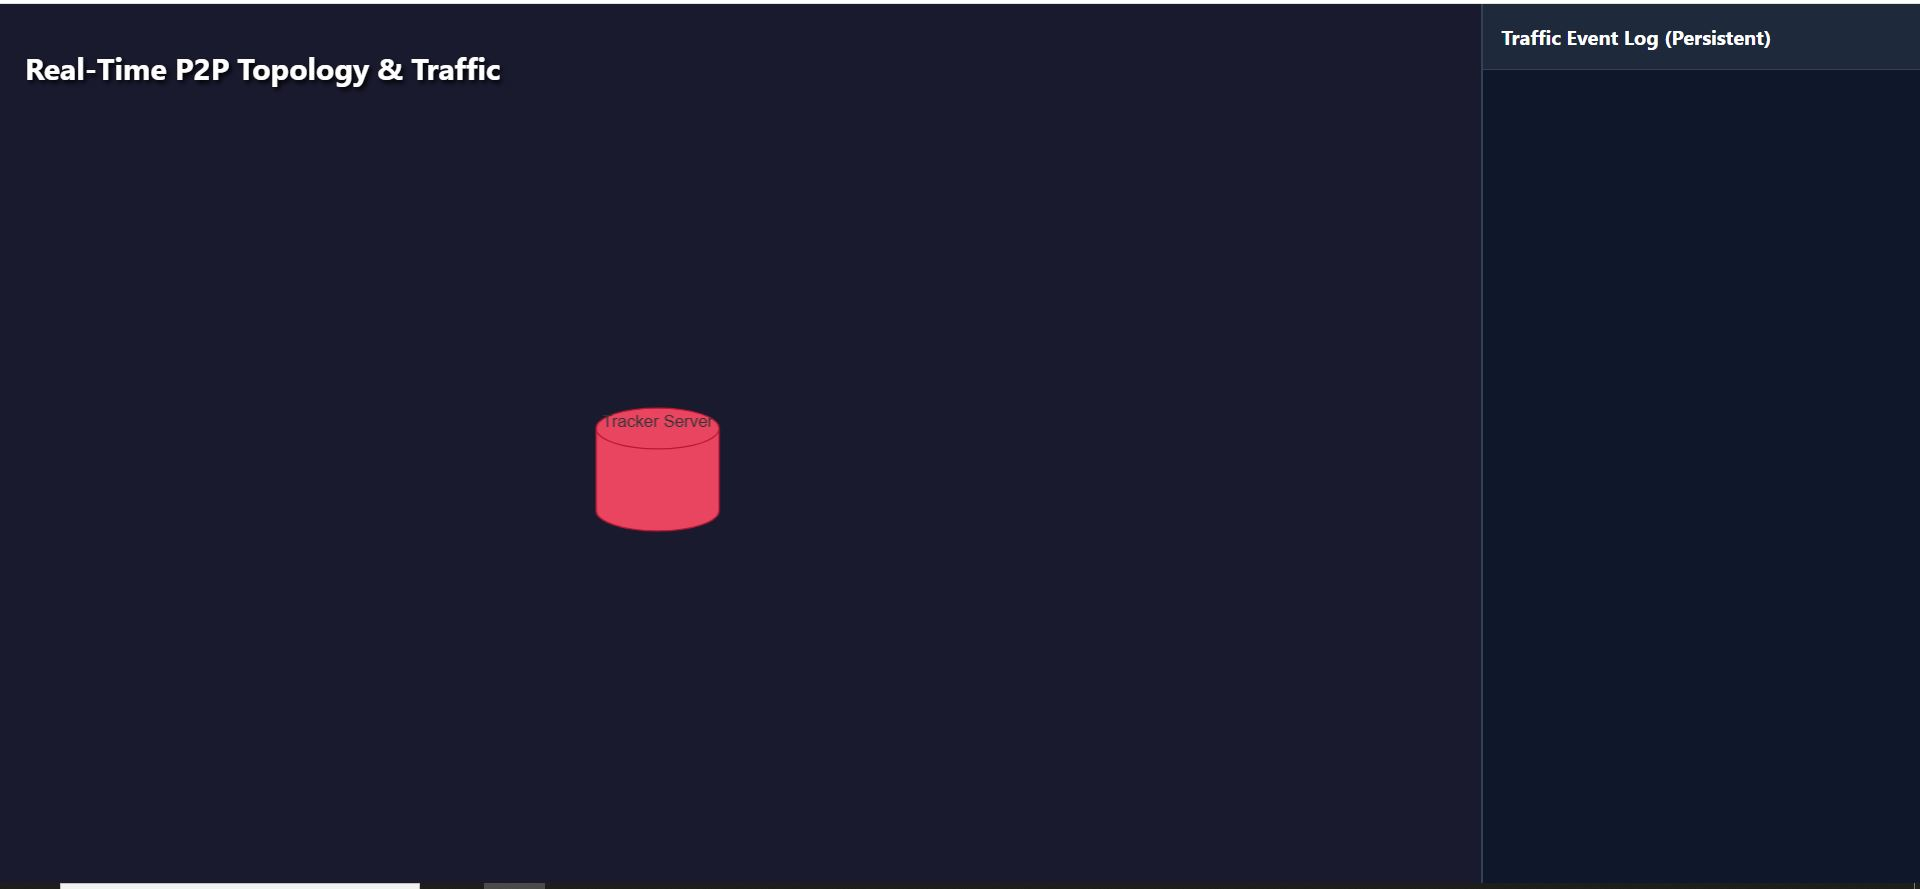
\includegraphics[width=0.8\textwidth]{Images/dashboard.JPG}
    \caption{Initial state of the dashboard before any peers join the network.}
    \label{fig:dash_empty}
\end{figure}

\subsection{Seeder Registration}
Next, we execute \texttt{peer.py 1}. This peer's workspace already contains the complete files defined in our first torrent. 
Upon startup, the client scans its local directory, verifies the integrity of the files, and automatically registers with the tracker as a Seeder. 
The dashboard dynamically updates to show the torrent swarm and the newly joined peer.

\begin{figure}[H]
    \centering
    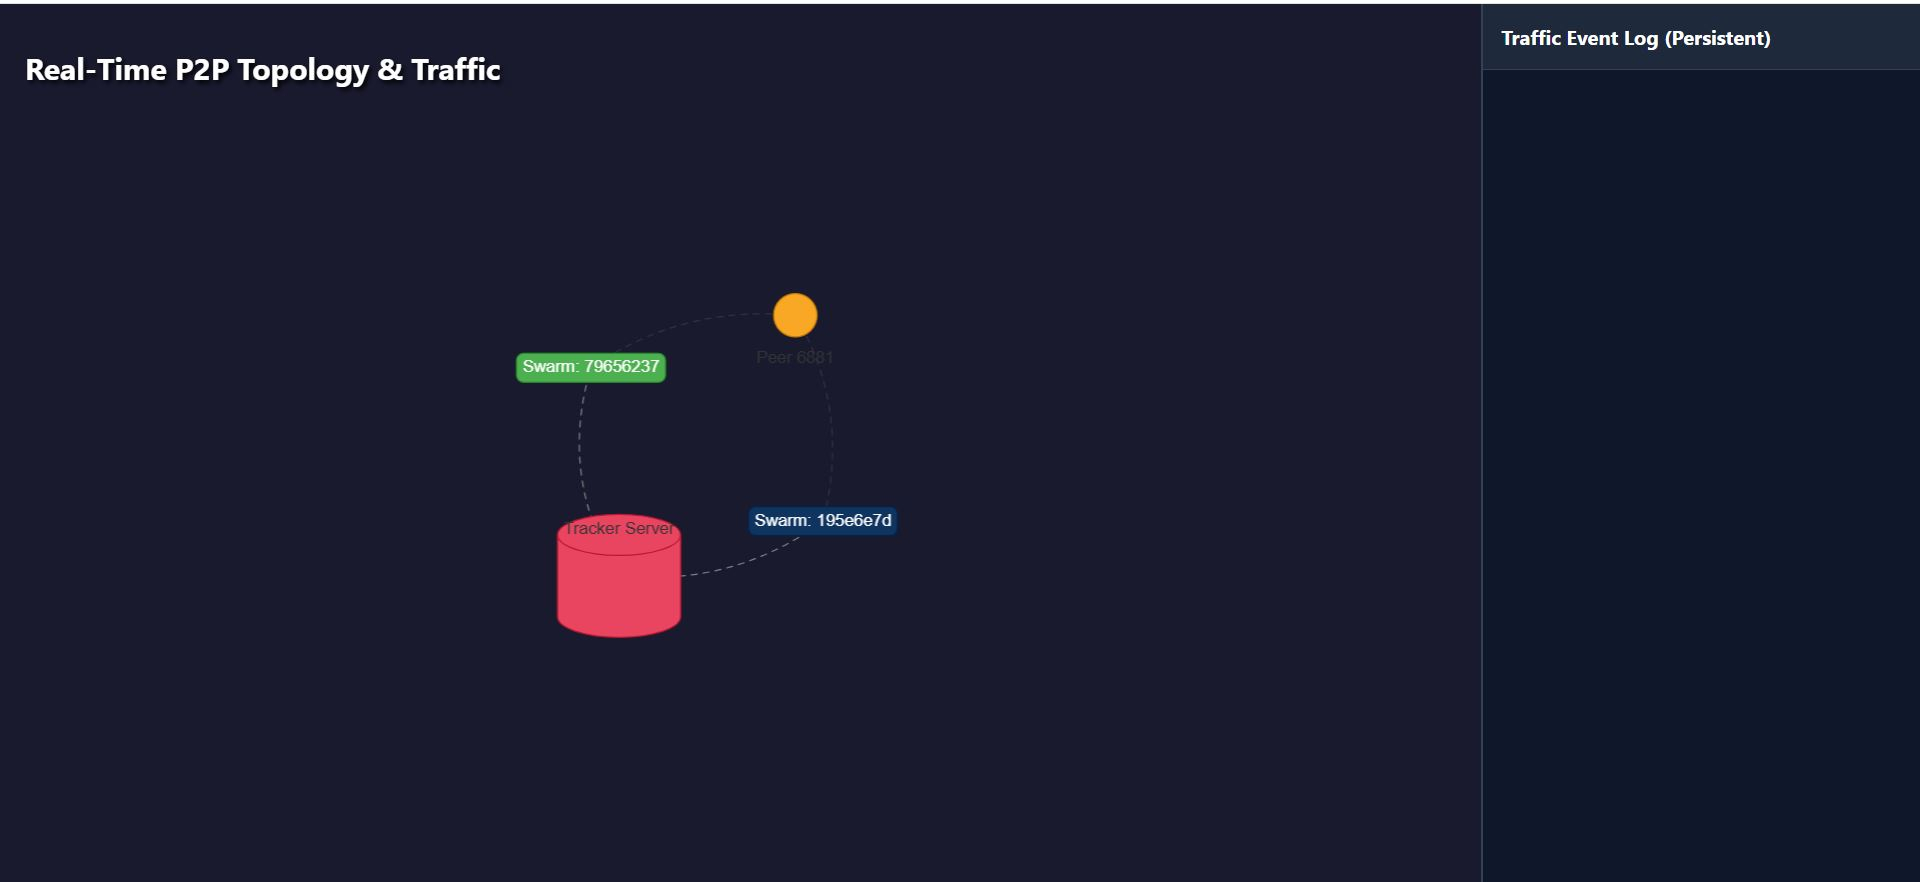
\includegraphics[width=0.8\textwidth]{Images/peer1.JPG}
    \caption{The dashboard displays Peer 1 joined as a seeder for the torrent swarm.}
    \label{fig:dash_seeder}
\end{figure}

\subsection{Leecher Joining and Data Transfer}
To simulate a download, a new client is launched by executing \texttt{peer.py 3}. Because this ID index was not used previously, the script generates a fresh, empty workspace directory named \texttt{workspace\_-AA0001-000000000003}. 

Within the internal terminal of Peer 3, the command \texttt{download 1} is issued to initiate the download process. The tracker introduces Peer 3 to Peer 1, handshakes are exchanged, and the piece transfer begins. 
The dashboard captures this rapid exchange of \texttt{REQ} and \texttt{PIECE} messages seamlessly.

\begin{figure}[H]
    \centering
    % ردیف اول
    \begin{subfigure}[b]{0.48\textwidth}
        \centering
        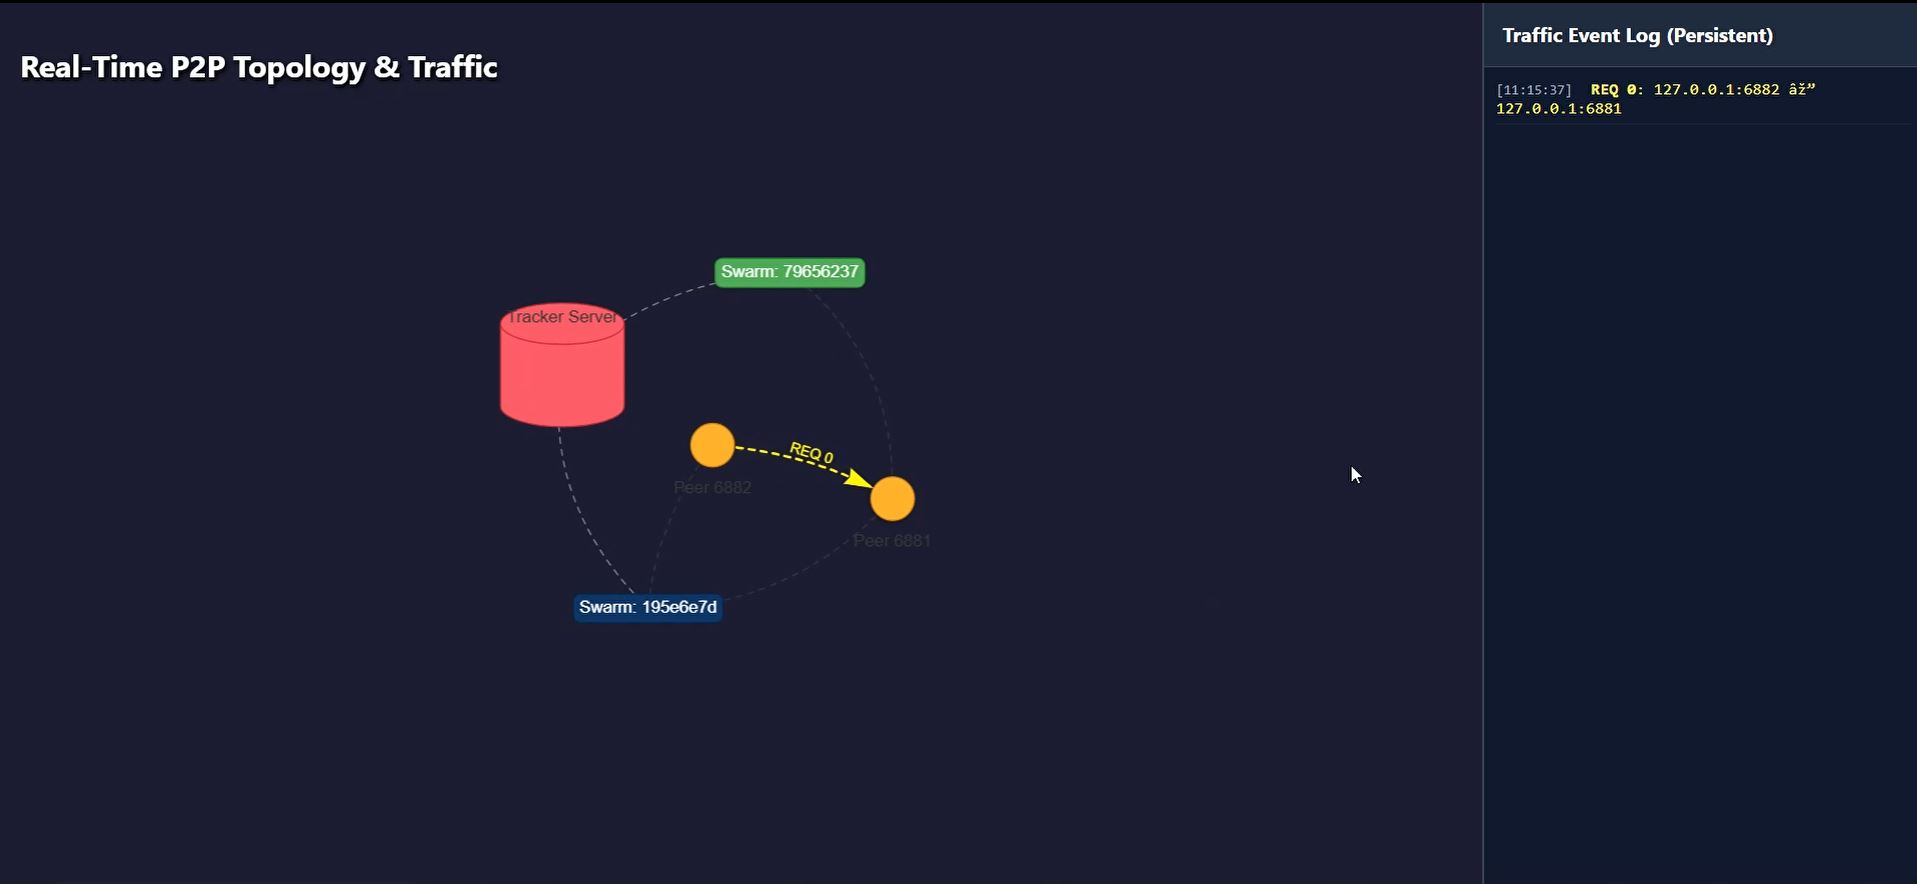
\includegraphics[width=\textwidth]{Images/1.jpg}
        \caption{Initiating data transfer: Peer 3 requesting the first piece (REQ 0).}
    \end{subfigure}
    \hfill
    \begin{subfigure}[b]{0.48\textwidth}
        \centering
        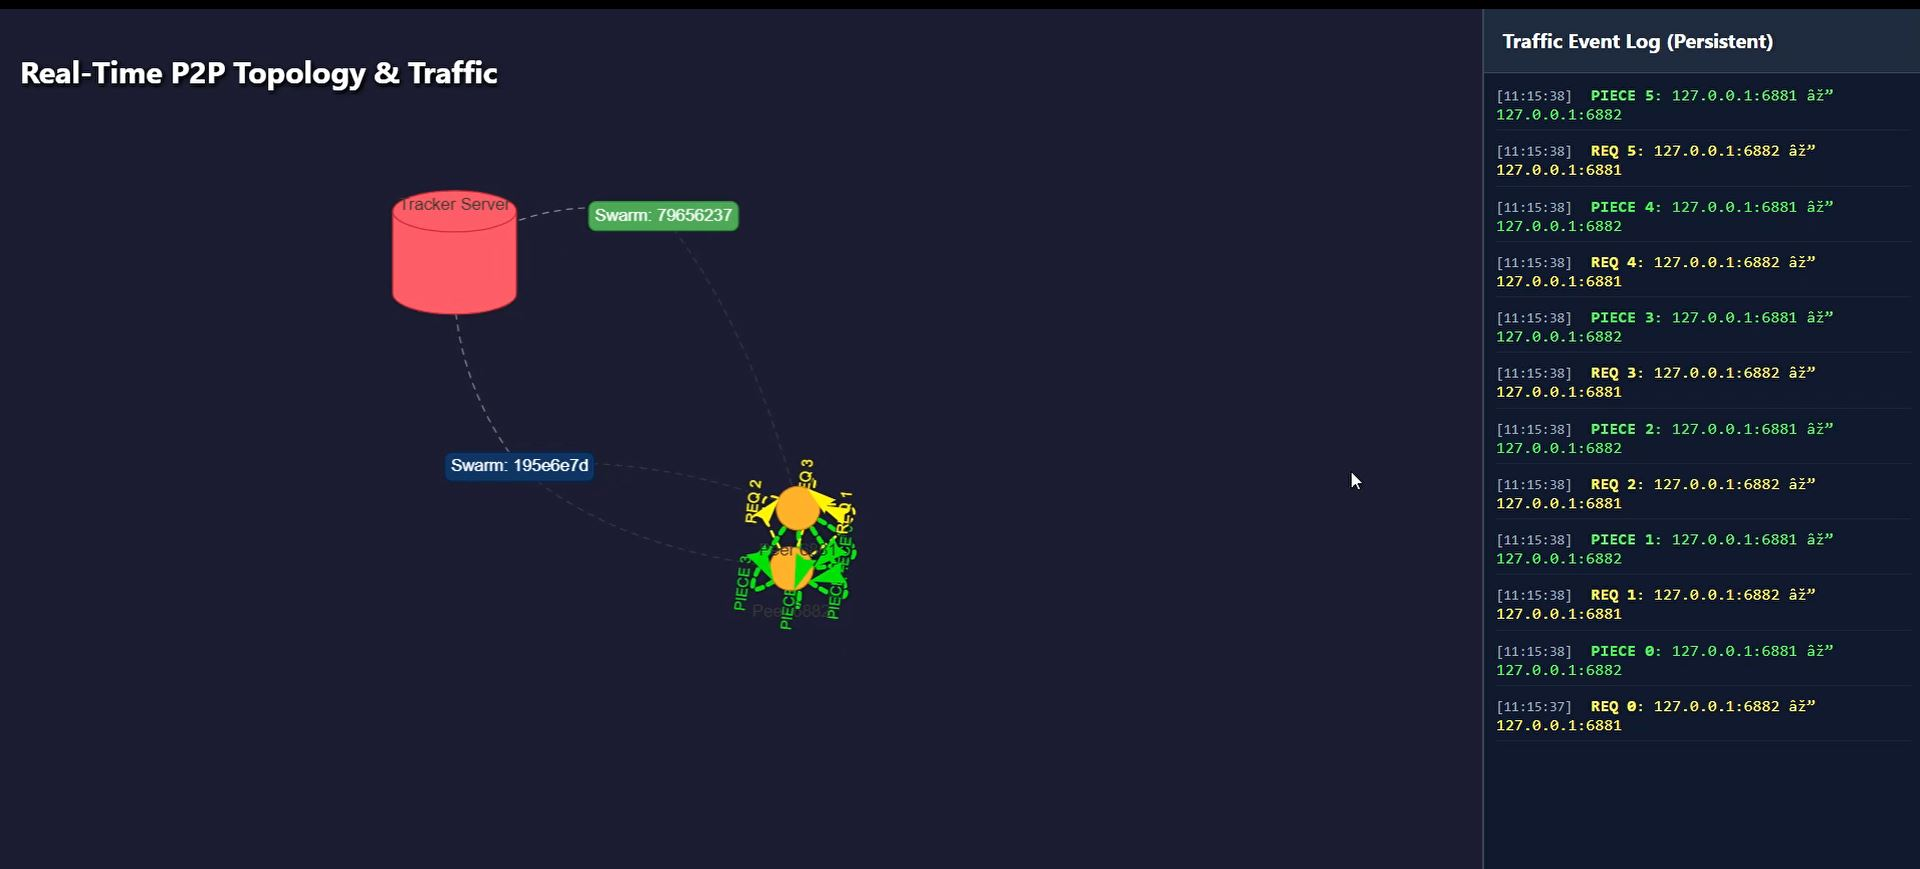
\includegraphics[width=\textwidth]{Images/2.jpg}
        \caption{Continuous exchange: Multiple REQ and PIECE messages being transmitted.}
    \end{subfigure}
    
    \vspace{1em} % ایجاد فاصله عمودی بین ردیف‌ها
    
    % ردیف دوم
    \begin{subfigure}[b]{0.48\textwidth}
        \centering
        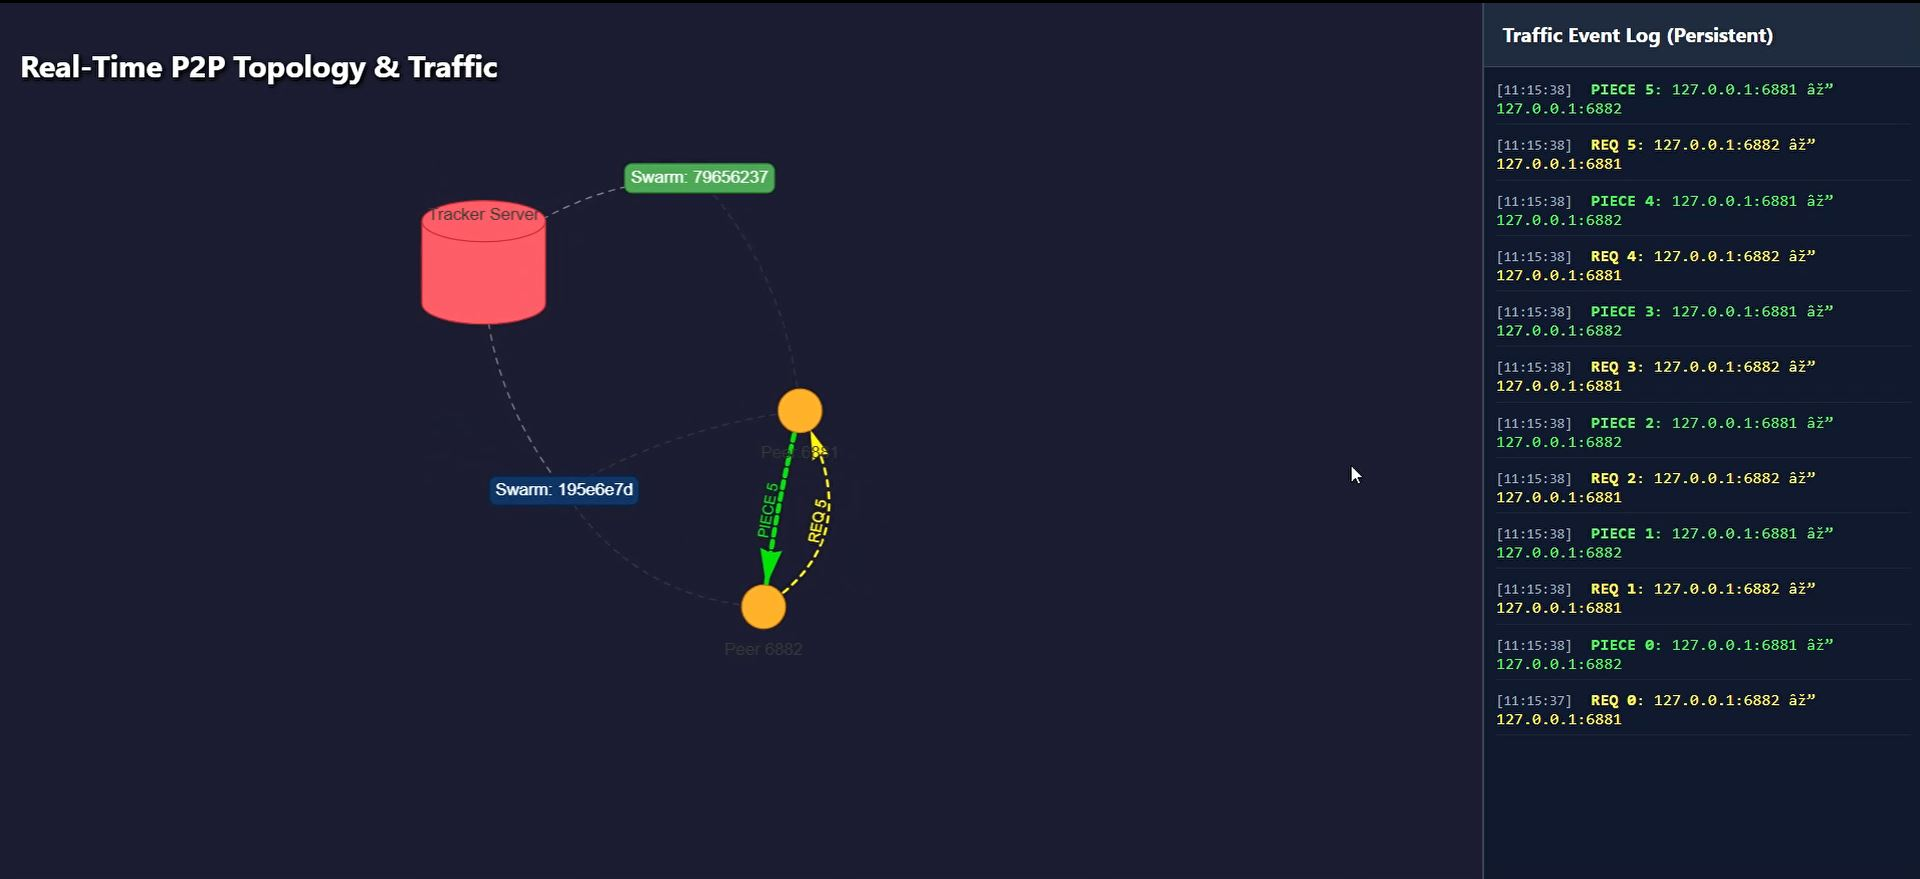
\includegraphics[width=\textwidth]{Images/3.jpg}
        \caption{Nearing completion: Transmission of the final REQ and PIECE.}
    \end{subfigure}
    \hfill
    \begin{subfigure}[b]{0.48\textwidth}
        \centering
        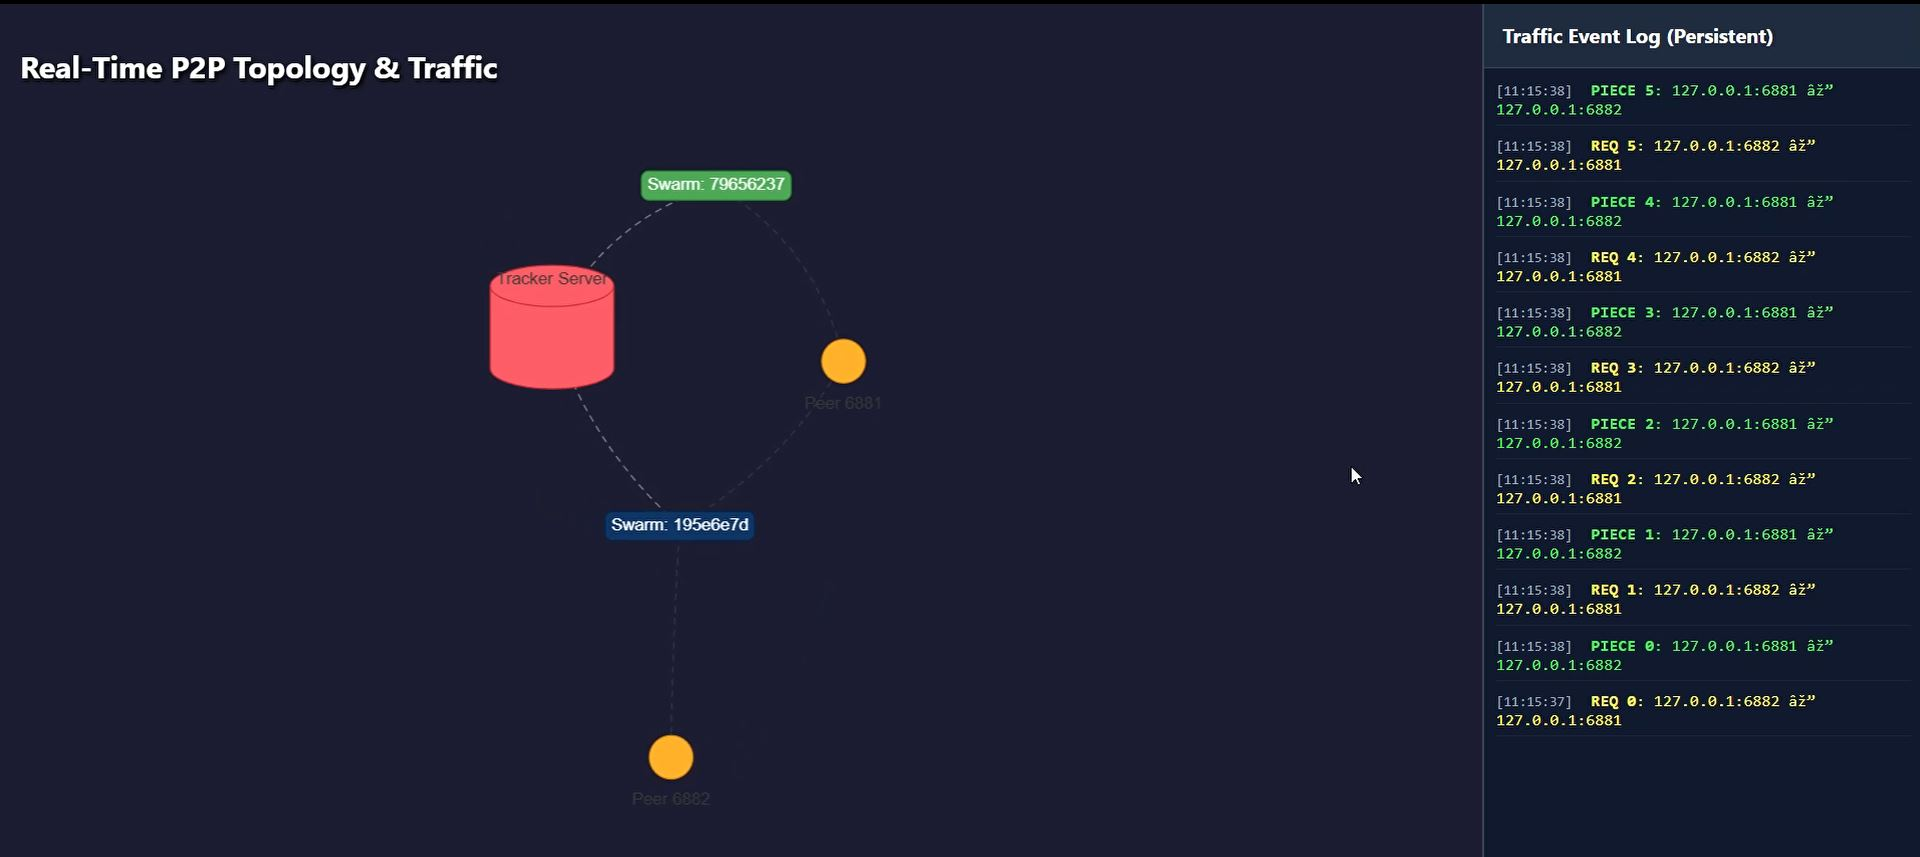
\includegraphics[width=\textwidth]{Images/4.jpg}
        \caption{Download complete: The peer successfully acquired all file pieces.}
    \end{subfigure}
    
    \vspace{1em} 
    
    % ردیف سوم (تک عکس وسط‌چین)
    \begin{subfigure}[b]{0.48\textwidth}
        \centering
        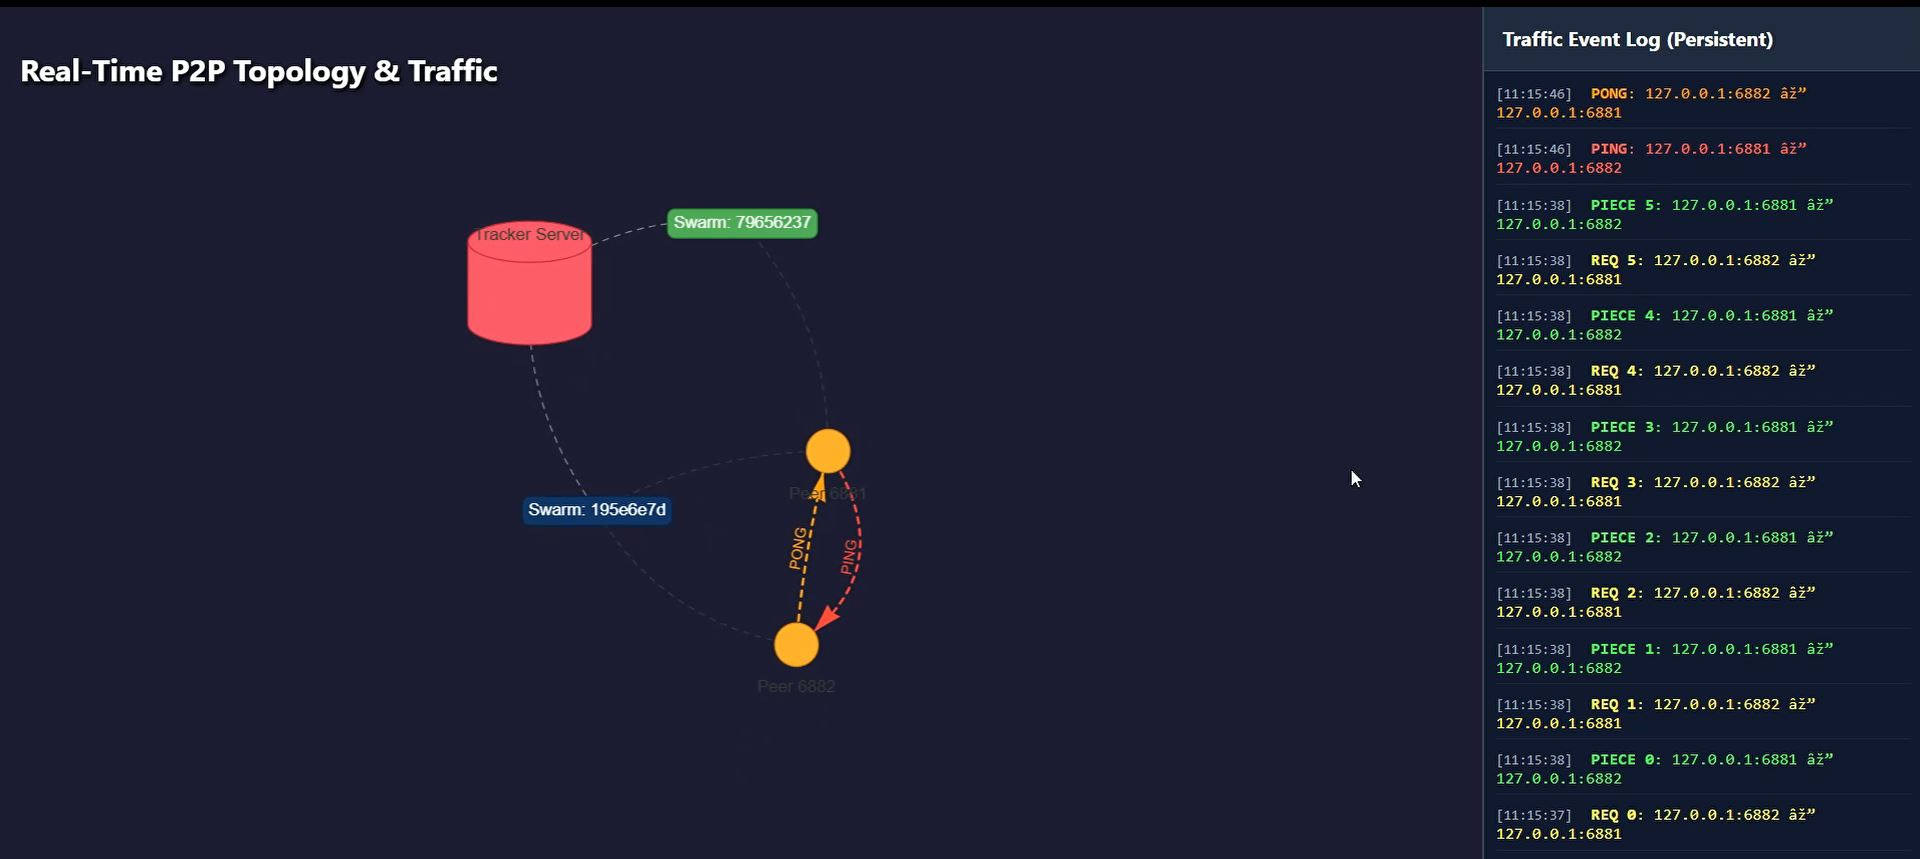
\includegraphics[width=\textwidth]{Images/5.jpg}
        \caption{Swarm maintenance: Periodic PING and PONG heartbeats between peers.}
    \end{subfigure}
    
    \caption{Chronological progression of the data transfer phase and subsequent swarm network maintenance.}
    \label{fig:dash_transfer_sequence}
\end{figure}

\subsection{Graceful Disconnection}
Once the transfer is complete, or if a user decides to leave the swarm, the \texttt{exit} command is executed in the peer's terminal. 
The peer transmits a \texttt{stopped} event to the tracker. The tracker successfully deregisters the peer from its internal database, and the node is subsequently cleared from the dashboard topology.

\section{Wireshark and Network Observation}
To verify the application level implementation and observe the network stack behavior, Wireshark was used to capture the local loopback traffic.

\subsection{Tracker Communication}
By filtering the traffic on \texttt{tcp.port == 8000}, the HTTP communication between the peers and the tracker is isolated. 
As shown in Figure \ref{fig:ws_tracker}, the peer successfully sends an HTTP \texttt{GET} request containing the URL encoded \texttt{info\_hash}, \texttt{peer\_id}, and \texttt{port}. 
The tracker processes this event and responds with an HTTP \texttt{200 OK} containing the bencoded dictionary of the swarm state.

\begin{figure}[H]
    \centering
    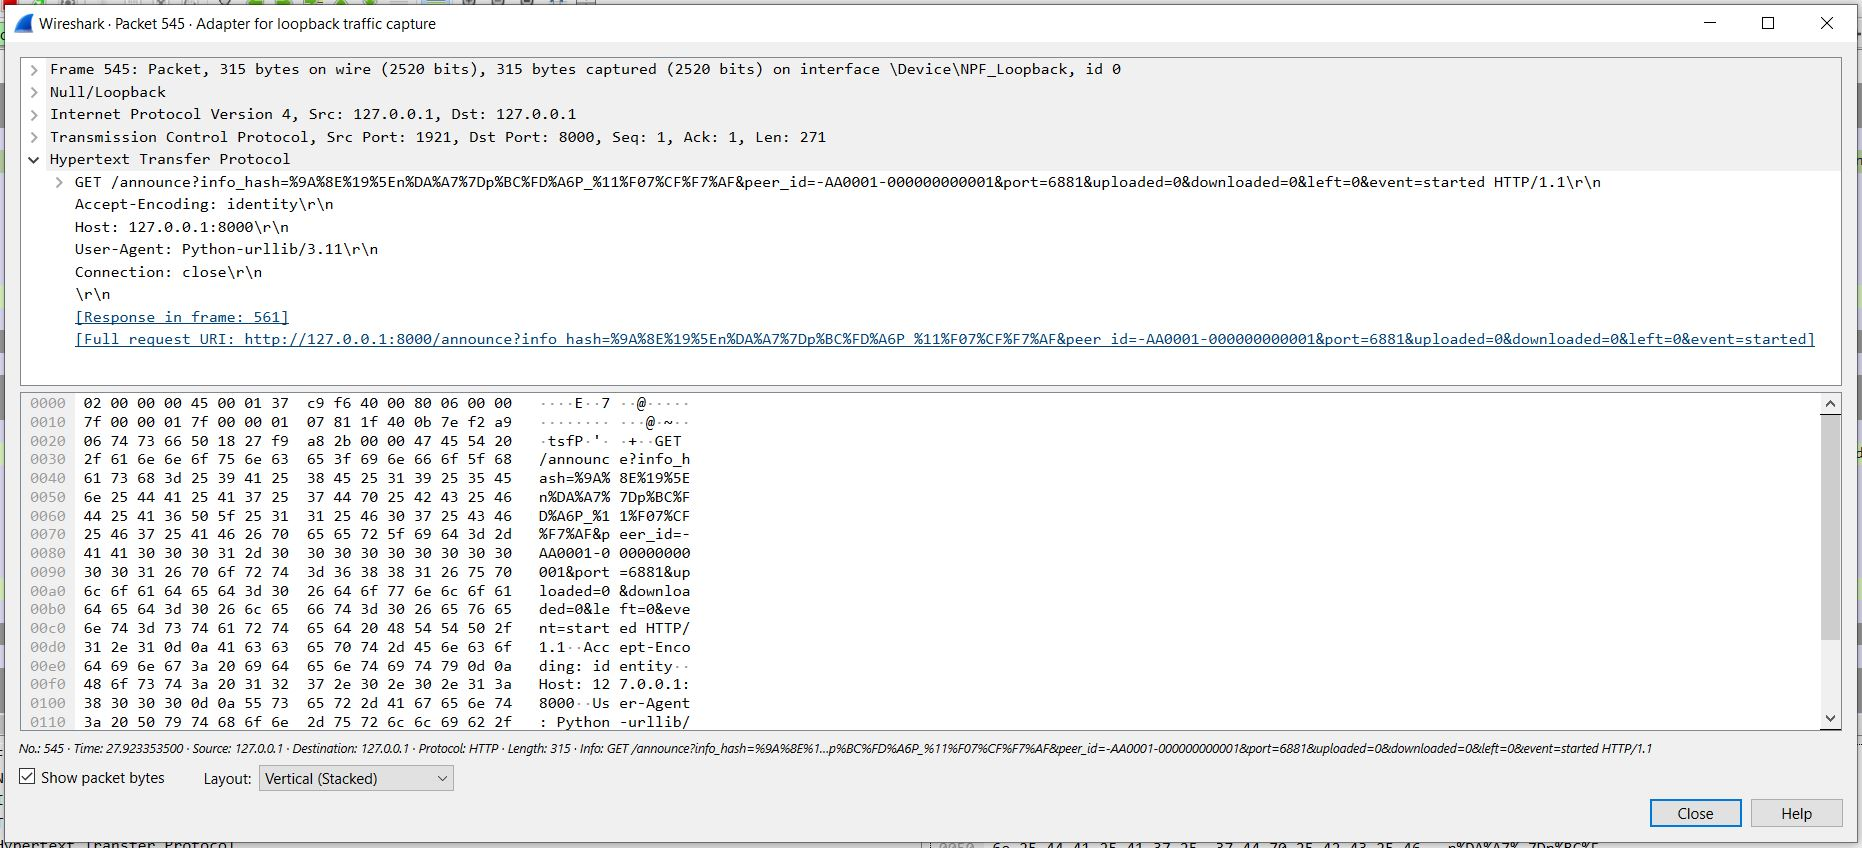
\includegraphics[width=0.9\textwidth]{Images/w1.JPG}
    \caption{Wireshark capture of the HTTP GET request sent to the Tracker's /announce endpoint.}
    \label{fig:ws_tracker}
\end{figure}

\subsection{Peer-to-Peer TCP Fragmentation}
Filtering the capture for \texttt{tcp.port >= 6881} reveals the direct communication between peers. 
A critical observation regarding the BitTorrent protocol is the distinction between application level pieces and network level packets. 

In this project, the \texttt{piece length} is configured to 256 KiB. Because a single Ethernet MTU is typically 1500 bytes, the operating system's network stack must fragment a single \texttt{PIECE} message into multiple sequential TCP packets. 
Figure \ref{fig:ws_tcp} demonstrates this behavior, showing numerous \texttt{[TCP segment of a reassembled PDU]} packets. The peer implementation handles this seamlessly by utilizing a continuous \texttt{recv\_all} buffer loop to reconstruct the 
complete payload independent of TCP boundaries.

\begin{figure}[H]
    \centering
    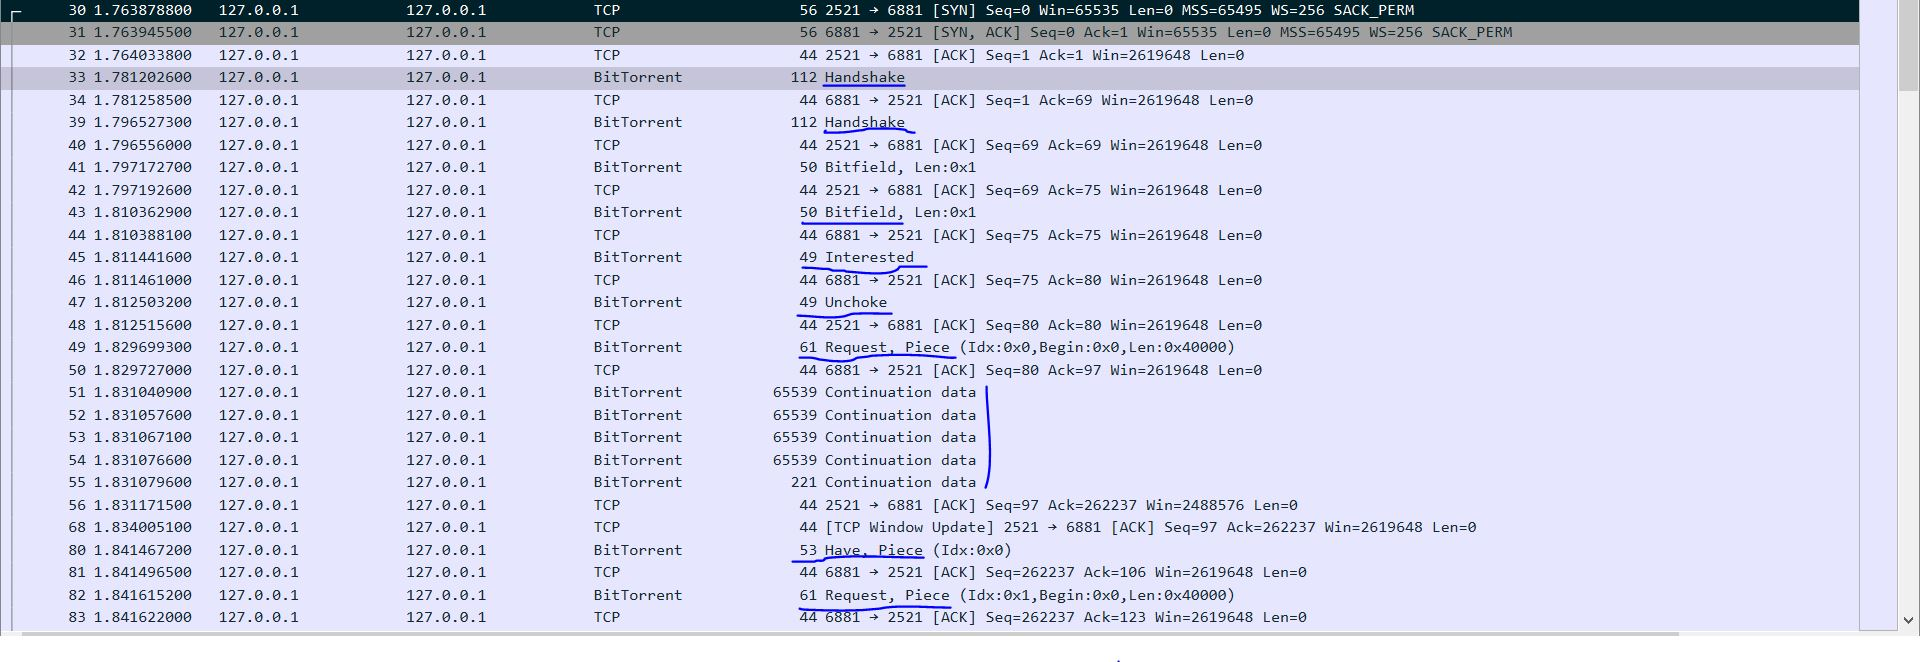
\includegraphics[width=0.9\textwidth]{Images/w2.JPG}
    \caption{Observation of TCP packet fragmentation for a large BitTorrent PIECE transmission.}
    \label{fig:ws_tcp}
\end{figure}

\end{document}